\section{Authentication and authorization}
Authentication and authorization processes are implemented using the secure OAuth 2.0 protocol \cite{oauth}. The whole procedure is based on communication and data exchange between four roles and components: the resource owner(user) the client app, the authorization server and the authorization microservice.

\subsection{OAuth protocol}
OAuth protocol is a modern industry-standard protocol for authorization. 
In general, the OAuth protocol enables users to provide a client with secure access to server resources and without a need for users to share their credentials directly with an application they want to access. OAuth is widely used by major companies to allow users to grant access to their resources to trusted third-party applications. \cite{oauth} This protocol is also obviously suitable for university applications and the BI-DBS portal in particular.

\subsection{Tokens} Token in this context is a string that has some value for authentication and authorization processes. In the implementation, the client gets the authorization code from the authorization server and exchanges it for access and refresh tokens with the server. 

\subsubsection{Access token}
The OAuth protocol uses an access token to represent the authorization status in the application. The access token is a short-time living token used to verify the user's access to the application. \cite{access-token} An access token is sent in every HTTP request made to the server. Thus the server can verify if the token is valid and then complete a request. It can be used for communication with the application server until that token expires. The expiration time is set to one hour. \\ 
The implementation uses a JWT token type for creating the access token. 
 
\paragraph*{JWT token.} JSON web token(JWT) is a token type standard that allows securely transmitting JSON objects. It consists of three parts: header which specifies the algorithm used to sign the token, payload containing the data being sent and signature that validates the token's integrity and assures it has not been modified. \cite{jwt-token}

\begin{figure}[hp]
\centering
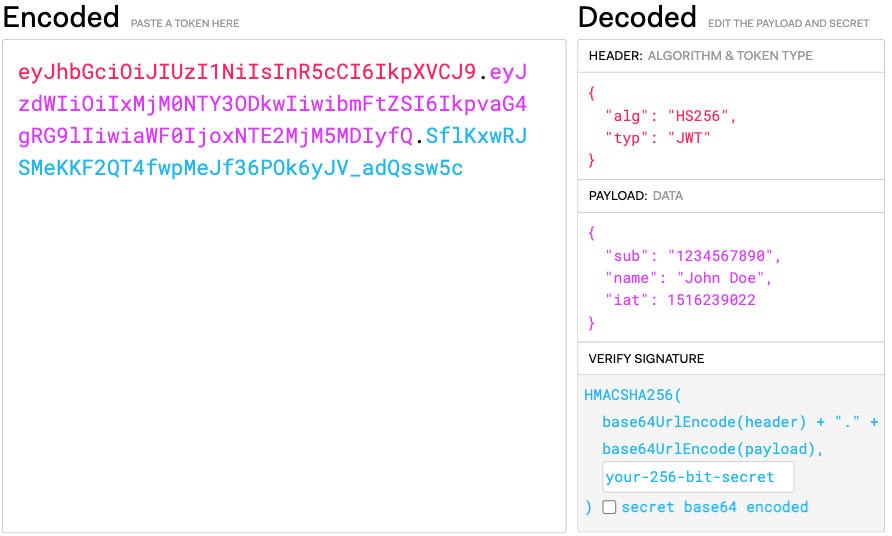
\includegraphics[scale=0.38]{../png/jwt_token.png}
\caption{Example of encoded and decoded JWT token from jwt.io. \cite{jwt-token}}
\label{jwt}
\end{figure}



\subsubsection{Refresh token} Refresh token is a type of token used for requesting a new access token when the current one expires. It is a long-time living token because it is meant to live longer than an access token due to its existence purpose. With the help of a refresh token user does not need repeatedly log in every hour which helps to improve user experience. \cite{refresh-token}


\subsection{Authorization server} The authorization server is a key component of the authorization and authentication processes based on the OAuth 2.0 protocol. 
For the authentication and authorization in the BI-DBS portal, we use the faculty's authorization server called Zuul OAAS. It is open-source and available for anybody from CTU. \cite{auth-server} Zuul OAAS provides three endpoints:

\begin{itemize}
    \item \emph{Authorization endpoint: /oauth/authorize.} It is used for the authentication and authorization processes of a user. It displays the login form for a user and after the submission of that form, it validates credentials and in a case of success does a redirect back to the BI-DBS client app server with the authorization code. 
    \item \emph{Token Endpoint: /oauth/token.} This endpoint provides us with two important functionalities:
        \begin{itemize}
            \item Exchanging authorization code from the authorization endpoint for access and refresh tokens.
            \item Generating new access token by accepting the refresh token.
        \end{itemize}
   \item \emph{Check Token Endpoint: /oauth/check\_token.} For controlling the validity of the token, the authorization server provides this endpoint which checks the token for being valid.
\end{itemize}

\noindent With the use of these endpoints we have constructed the authentication and authorization processes, which are more deeply described in \ref{sec425} and shown in Figure \ref{access}.


\subsection{Apps manager} To communicate with the authorization server, the application must be registered in the Apps Manager \cite{app-manager}. For further communication with the server we will need three parameters: client id, client secret and redirect URL. The first two parameters are generated by the app manager. These are simplified login and password for our application. But the redirect URL can be set to the URL we want, this URL will be used for the redirect back to our application after the successful authorization of a user. These parameters are used as a part of the HTTP requests, that frontend and backend send to the authorization server. 

\begin{figure}[hp]
\centering
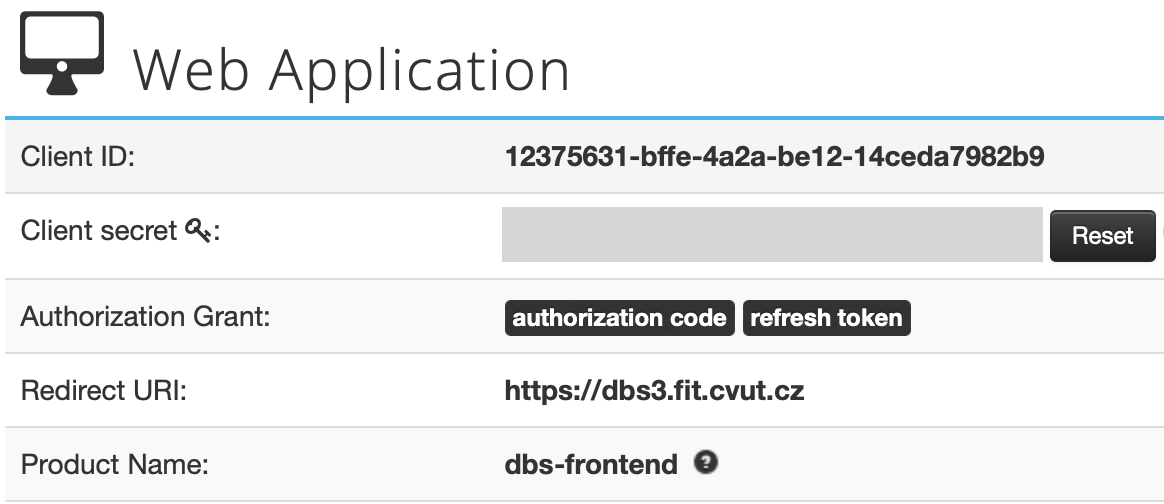
\includegraphics[scale=0.52]{../png/app_manager.png}
\caption{The example of the application registry in the App Manager \cite{app-manager}}
\label{appm}
\end{figure}


\subsection{Authentication and authorization flow}\label{sec425} For better visualization I have provided the implicit flow of the implemented services and a sequential diagram in Figure \ref{access}.\\

\noindent \textbf{Explicit flow:}

\begin{enumerate}
    \item Unauthorized user is trying to access the application and access validation redirects a user to the login page.
    \item By clicking on the login button user gets transferred to the page provided by the authorization server with a form for submitting credentials.
    \item After submitting credentials authorization server redirects the user back to the BI-DBS client with an authorization code which the client exchanges with the backend for the JWT access and refresh tokens.
    \item Finally the user is redirected to the page they wanted to access.
\end{enumerate}

\begin{figure}[hp]
\centering
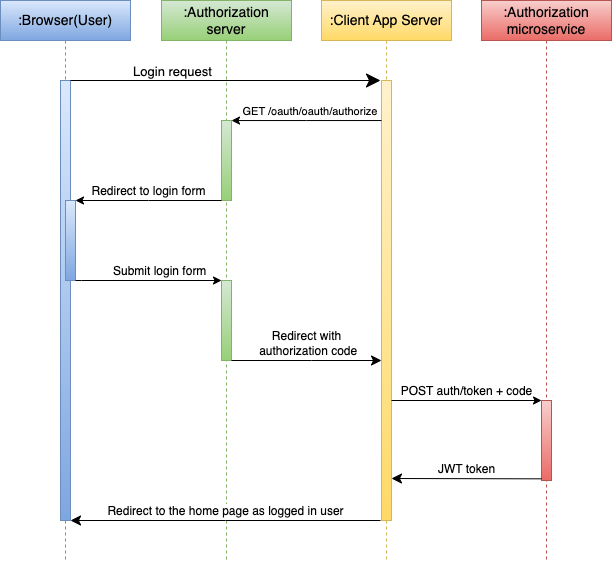
\includegraphics[scale=0.56]{../png/generate_token.png}
\caption{Sequential diagram of generating an access token}
\label{access}
\end{figure}



\subsection{Refresh token flow} Another very important part of the implementation is refreshing the access token with the usage of the refresh token. A user does not know about that process and does not participate in it. This process replaces the constant logging in by a user, which improves security since a user does not need to enter credentials repeatedly and also does not annoy or interrupt a user. The explicit flow and sequential diagram of the token refreshing process in Figure \ref{refresh} are provided for showing the implementation details.\\

\noindent \textbf{Explicit flow:}

\begin{enumerate}
    \item A user who has already been authorized in the application is trying to make a request. However, the access token has expired and cannot be used anymore for the requests.
    \item The client detects that the access token has expired and sends a request to the authorization microservice for a new access token in exchange for the current access token and the refresh token.
    \item After receiving a new access token client completes the request for a user with the usage of that access token.
\end{enumerate}

\begin{figure}[hp]
\centering
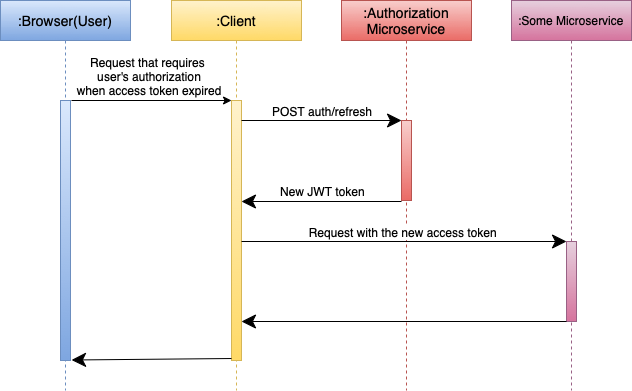
\includegraphics[scale=0.6]{../png/refresh_token.png}
\caption{Sequential diagram of refresh an access token using refresh token}
\label{refresh}
\end{figure}
